%%%%%%%%%%%%%%%%%%%%%%%%%%%%%%%%%%%%%%%%%%%%%%%%%%%%%%%%%%%%%%%%%%%%%%%%%%%%%%%%%%%%
% Do not alter this block (unless you're familiar with LaTeX
\documentclass{article}
\usepackage[margin=1in]{geometry} 
\usepackage{amsmath,amsthm,amssymb,amssymb,amsfonts, fancyhdr, color, comment, graphicx, environ}
\usepackage{mathrsfs}

\usepackage{xcolor}
\usepackage{mdframed}
\usepackage[shortlabels]{enumitem}
\usepackage{indentfirst}
\usepackage{hyperref}
\hypersetup{
    colorlinks=true,
    linkcolor=blue,
    filecolor=magenta,      
    urlcolor=blue,
}


\pagestyle{fancy}

\newcommand{\aboverightarrow}[1]{\xrightarrow[]{#1}}

\newenvironment{problem}[2][Problem]
    { \begin{mdframed}[backgroundcolor=gray!20] \textbf{#1 #2} \\}
    {  \end{mdframed}}

% Define solution environment
\newenvironment{solution}
    {\textit{Solution:}}
    {}
    \newcommand{\indep}{\perp \!\!\! \perp}
    \renewcommand\qedsymbol{$\blacksquare$}
\newcommand{\norm}[1]{\left\lVert#1\right\rVert}
\newcommand{\seminorm}[1]{\left [#1\right]}
\newcommand{\ts}{\textsuperscript}
\usepackage{scalerel}[2014/03/10]
\usepackage[usestackEOL]{stackengine}
\def\avint{\,\ThisStyle{\ensurestackMath{%
  \stackinset{c}{.2\LMpt}{c}{.5\LMpt}{\SavedStyle-}{\SavedStyle\phantom{\int}}}%
  \setbox0=\hbox{$\SavedStyle\int\,$}\kern-\wd0}\int}
\def\ddashint{\,\ThisStyle{\ensurestackMath{%
  \stackinset{c}{.2\LMpt}{c}{.5\LMpt+.2\LMex}{\SavedStyle-}{%
    \stackinset{c}{.2\LMpt}{c}{.5\LMpt-.2\LMex}{\SavedStyle-}{%
      \SavedStyle\phantom{\int}}}}\setbox0=\hbox{$\SavedStyle\int\,$}\kern-\wd0}\int}

\newcommand{\skipline}{$ \ $}

\newcommand{\reals}{\mathbb R}
\newcommand{\ints}{\mathbb Z}
\newcommand{\normal}{\trianglelefteq}
\newcommand{\onormal}{\trianglerighteq}

\newcommand{\subgroup}{\leqslant}

\newcommand{\sigalg}{\mathscr A}
\newcommand{\setsequence}{ \{ E_n \}_{n=1}^{\infty} }
\newcommand{\unionsetsequence}{ \bigcup_{i=1}^{\infty}  A_i }
\newcommand{\intersectionsetsequence}{ \bigcap_{i=1}^{\infty}  A_i }
\newcommand{\measureablespace}{(X, \sigalg)}
\newcommand{\measurespace}{(X, \sigalg, \mu)}
\newcommand{\borelspace}{\mathscr{B}(X)}
\newcommand{\lebesguemeasurespace}{(X, \borelspace, \lambda)}
\newcommand{\schwartzspace}{\mathcal S(\mathbb R^n)}
\newcommand{\temperedspace}{\mathcal S'(\mathbb R^n)}

\newcommand{\measure}{\mu: \sigalg \rightarrow [0, + \infty]} 
\newcommand{\outermeasure}{\mu: \mathbb{P}(X) \rightarrow [0, + \infty]} 
\newcommand{\convergesinmeasure}{\xrightarrow[\mu]{}} 
\newcommand{\convergesinLp}{\xrightarrow[L^p]{}} 

\newcommand{\convergesinschwartz}{\xrightarrow[]{\mathcal S}} 

\renewcommand{\qed}{\quad\qedsymbol}
\setlength\parindent{0pt}

% prevent line break in inline mode
\binoppenalty=\maxdimen
\relpenalty=\maxdimen

%%%%%%%%%%%%%%%%%%%%%%%%%%%%%%%%%%%%%%%%%%%%%
%Fill in the appropriate information below
\lhead{Greg DePaul}
\rhead{Stats 206} 
\chead{\textbf{Homework 3  Due: 20 October 2022}}
%%%%%%%%%%%%%%%%%%%%%%%%%%%%%%%%%%%%%%%%%%%%%

\begin{document}

\begin{problem}{1}
Submitted as a  Markdown file. 
\end{problem}

\begin{problem}{2}
\textbf{Q-Q plots.} For each of the following Q-Q plots, describe the distribution of the data (whether it is Normal or heavy tailed, etc.).


\begin{center}
  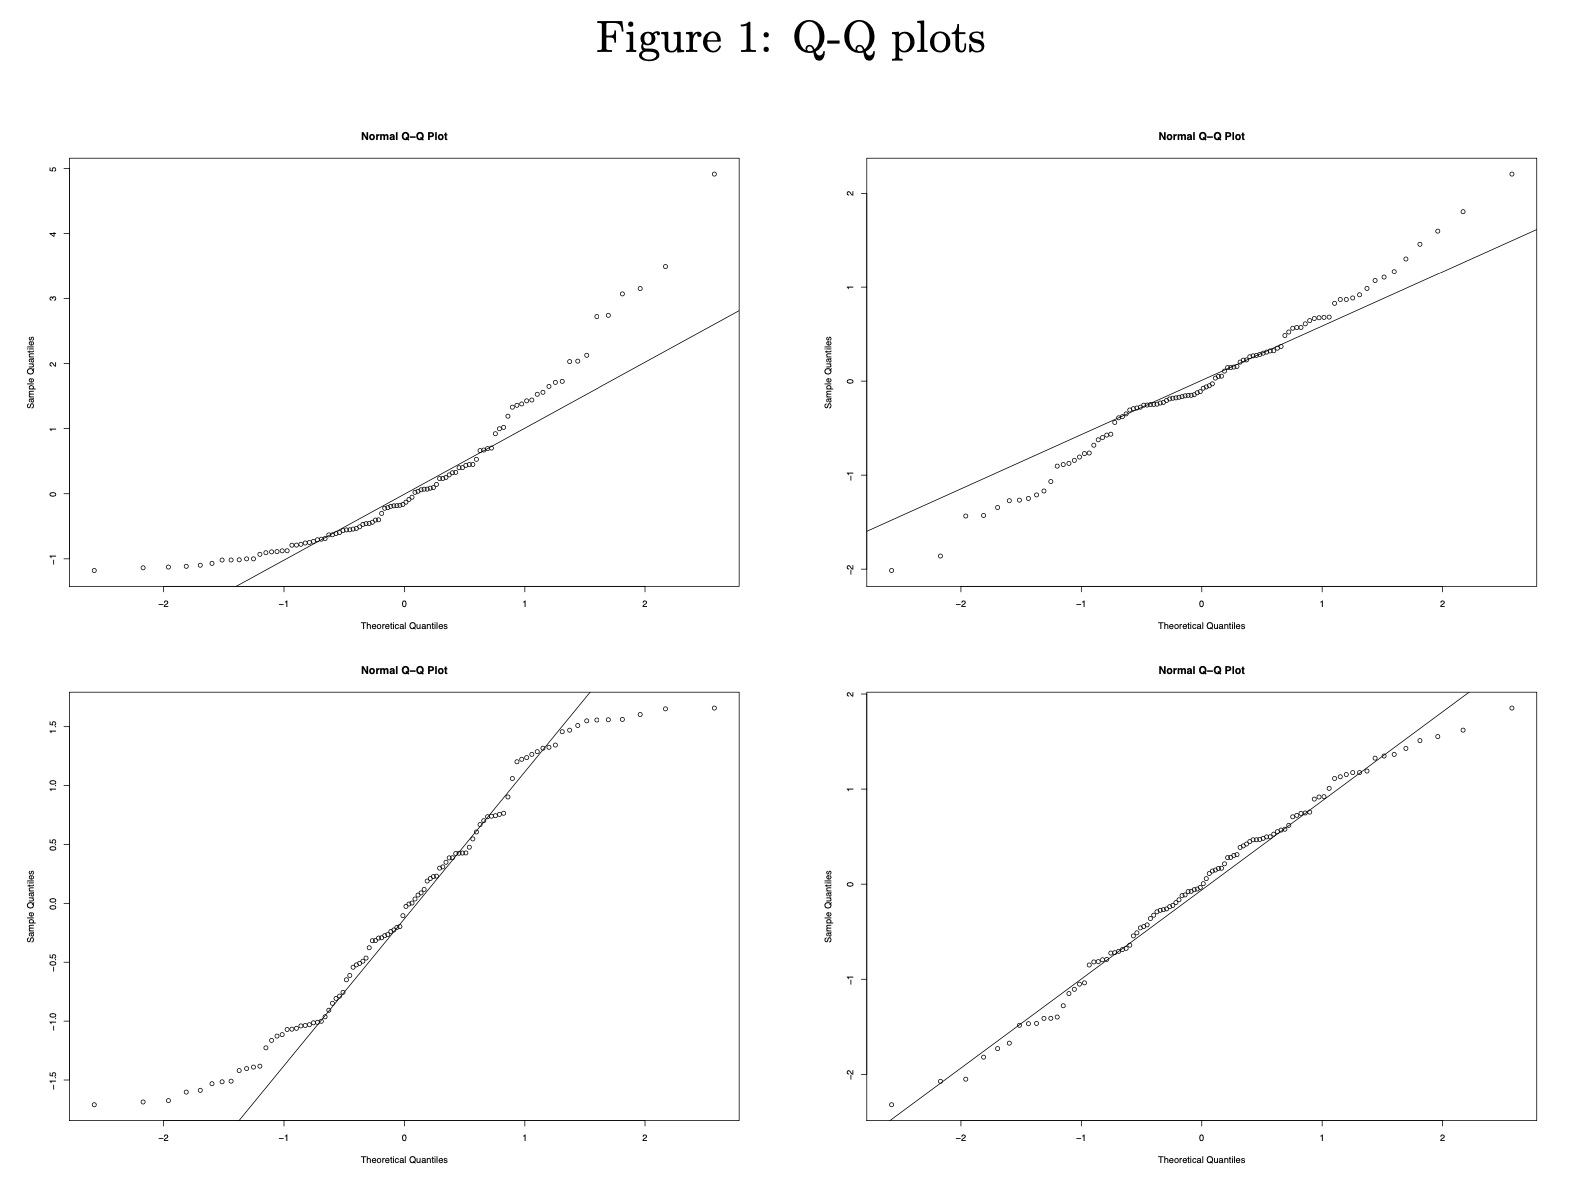
\includegraphics[width=6in]{fig1.png}
\end{center}
\end{problem}
\begin{solution}
\begin{enumerate}[(a)]
\item This relationship is right-skewed. 
\item This relationship is heavy tailed. 
\item This relationship is heavy tailed. 
\item This looks very normal, with some possible outliers at the percentile ends. 
\end{enumerate}
\end{solution}


\begin{problem}{3}
\textbf{Coefficient of determination.} Show that 
$$R^2 =r^2, r= \text{sign}\{\beta_1\} \sqrt{R^2}$$
where $R^2$ is the coefficient of determination when regressing $Y$ onto $X$ and $r$ is the sample correlation coefficient between $X$ and $Y$.
\end{problem}
\begin{solution}
Observe, 

$$R^2 = \frac{SSR}{SSTO} = \frac{\beta_1^2 \left (\sum_{i = 1}^n (X_i - \overline{X})^2 \right)^2}{\sum_{i = 1}^n (Y_i - \overline{Y})^2} =  \frac{\left [ \sum_{i = 1}^n (X_i - \overline{X}) (Y_i - \overline{Y}) \right]^2}{ \left (\sum_{i = 1}^n (X_i - \overline{X}) \right) \left (\sum_{i = 1}^n (Y_i - \overline{Y})^2 \right) } = r^2$$

and since 
$$sign(r) = sign( \sum_{i = 1}^n (X_i - \overline{X}) (Y_i - \overline{Y})) = sign(\beta_1)$$

we can conclude that

$$r= \text{sign}\{\beta_1\} \sqrt{R^2}$$
\end{solution}



\begin{problem}{4}
Confirm the formula for inverting a $2 \times 2$ matrix.
\end{problem}
\begin{solution}
\begin{align*}
\begin{pmatrix}
a & b \\
c & d 
\end{pmatrix}\left (  \begin{pmatrix}
d & -b \\
-c & a 
\end{pmatrix} 
\right ) &=\frac{1}{ad -bc} \begin{pmatrix}
a & b \\
c & d 
\end{pmatrix}  \begin{pmatrix}
d & -b \\
-c & a 
\end{pmatrix}  \\
&= \frac{1}{ad -bc} \begin{pmatrix}
ad - bc & -ab + ab \\
cd - cd & -bc + ad 
\end{pmatrix}\\
&= \frac{1}{ad -bc} \begin{pmatrix}
ad - bc & 0 \\
0 & ad -bc   
\end{pmatrix}\\
&= \begin{pmatrix}
1 & 0 \\
0 & 1
\end{pmatrix}
\end{align*}

%$$\iff \begin{pmatrix}
%ae + bg & af + bh \\
%ce + dg & cf + dh \\
%\end{pmatrix} = \begin{pmatrix}
%1 & 0 \\
%0 & 1 
%\end{pmatrix}$$
%$$\iff \begin{cases}
%ae + bg = 1\\
%af + bh = 0 \\
%ce + dg = 0\\
%cf + dh = 1
%\end{cases}$$
%
%$$\iff \begin{cases}
%ace + bcg = c\\
%acf + bch = 0 \\
%ace + adg = 0\\
%acf + adh = a
%\end{cases}$$
%
%$$$$

\end{solution}




\begin{problem}{5}
\textbf{Projection matrices.} Show the following are projection matrices, i.e., being symmetric and idempotent. What are the ranks of these matrices? Here $\bf{H}$ is the hat matrix from a simple linear regression model with $n$ cases (where the $X$ values are not all equal) , $\bf{I_n}$ is the $n \times n$ identify matrix, and $\bf{J_n}$ is the $n \times n$ matrix with all ones.
\begin{enumerate}[(a)]
\item $\bf{I_n}$$ - \bf{H}$
\item $\bf{I_n}$$ - \frac{1}{n} \bf{J_n}$
\item  $\bf{H}$$ - \frac{1}{n} \bf{J_n}$
\end{enumerate}
\end{problem}
\begin{solution}
\begin{enumerate}[(a)]
\item 
\begin{itemize}
\item \emph{Idempotent}: \begin{align*}
(I_n - H)^2 &= I_n^2 - X(X^TX)^{-1}X^T - X(X^TX)^{-1}X^T + X(X^TX)^{-1}X^T \cdot X(X^TX)^{-1}X^T \\
& =  I_n - 2 H + X\left [ (X^TX)^{-1}X^TX \right ](X^TX)^{-1}X^T \\
& =  I_n - 2 H + X(X^TX)^{-1}X^T \\
& =  I_n - 2 H +H \\
&= I_n - H
\end{align*}
\item \emph{Symmetric}: $(I_n - H)' = I_n' - H' = I_n - H$
\item \emph{Rank}: $n - 2$
\end{itemize}
\item 
\begin{itemize}
\item \emph{Idempotent}: $(I_n - \frac{1}{n} J_n)^2 = I_n^2 - 2 \frac{1}{n} J_n   + \frac{1}{n^2} \cdot \bf{1} \cdot \bf{1}^T \cdot \bf{1}\cdot \bf{1}^T =  I_n - 2 \frac{1}{n} J_n   + \frac{1}{n} J_n = I_n - \frac{1}{n} J_n $
\item \emph{Symmetric}: $(I_n - \frac{1}{n} J_n)' = I_n' - \frac{1}{n} J_n' = I_n - \frac{1}{n} (\bf{1}\cdot \bf{1}^T)^T =  I_n - \frac{1}{n} ((\bf{1}^T)^T \cdot \bf{1}^T  = I_n - \frac{1}{n} (\bf{1}\cdot \bf{1}^T = I_n - \frac{1}{n} J_n$
\item \emph{Rank}: $n - 1$ 
\end{itemize} 
\item \begin{itemize} 
\item \emph{Idempotent}: 
\begin{align*}
(H - \frac{1}{n} J_n)^2 &= H^2 - \frac{1}{n} H J_n - \frac{1}{n} J_n H + \frac{1}{n} J_n^2\\
&= H - \frac{1}{n} H J_n - \frac{1}{n} J_n H + \frac{1}{n} J_n\\
&= H - \frac{1}{n} X (X^T X)^{-1} X^T \bf{1} \bf{1}^T - \frac{1}{n} \bf{1} \bf{1}^T  X (X^T X)^{-1} X^T + \frac{1}{n} J_n
\end{align*}
\item \emph{Symmetric:} $(H - \frac{1}{n} J_n)' = H' -\frac{1}{n} J_n' = H - \frac{1}{n} J_n $
\item \emph{Rank:} 1 
\end{itemize}
\end{enumerate}
\end{solution}



\begin{problem}{6}
Under the simple linear regression model, using matrix algebra, show that:
\begin{enumerate}[(a)]
\item The residual vector $\bf{e}$ is uncorrelated with the fitted values vector $\bf{\hat Y}$ and the LS estimator $\bf{\hat \beta}.$ \emph{Hint: If $\bf{Z}$ is an $r \times 1$ random vector, $\bf{A}$ is an $s \times r$ non-random matrix, and $\bf{B}$ is a $t \times r$ non-random matrix, then $Cov( \bf{AZ}, \bf{BZ}) = \bf{A\sigma^2\{Z\}B'}$.)}
\item With Normality assumption on the error terms, SSE is independent with the LS estimator $\bf{\hat \beta}$ and SSR.
\end{enumerate}
\end{problem}
\begin{solution}
\begin{enumerate}[(a)]
\item \begin{itemize}
\item Observe, 
\begin{align*}
Cov(e, \hat Y) &= Cov((1 - H) Y, H Y) \\
&= (1 - H) \sigma^2(Y) H^T\\ 
&= (1 - H) \sigma^2(Y) H \\
&= \sigma^2(Y) (1 - H)  H  & \text{since }  \sigma^2(Y) = \sigma^2 I \\
&=  \sigma^2(Y)(H - H^2) \\
&=   \sigma^2(Y)(H - H) \\
&= 0
\end{align*}
\item 
\begin{align*}
Cov(e, \hat \beta) &= Cov((I - H)Y, (X^TX)^{-1}X^T Y) \\
&= (I - H)\sigma^2(Y)X(X^TX)^{-T} & \text{since }  \sigma^2(Y) = \sigma^2 I \\
&=\sigma^2(Y) (I - X(X^TX)^{-1} X^T)X(X^TX)^{-T} \\
&=\sigma^2(Y) (X(X^TX)^{-T} - X(X^TX)^{-T}) \\
&= 0
\end{align*}
\end{itemize}
\item Define the function:
$$SSE = f(e) = e^Te = \norm{(I - H)Y}_2$$
Therefore, if we let $g = id : \mathbb R^n \rightarrow \mathbb R$, then we see that by the fact that if two sets of random variables, say $(Z_1, \ldots, Z_s)$ and $(W_1,\ldots ,W_t)$, are independent with each other, then their functions, say $f(Z_1, \ldots, Z_s)$ and $g(W_1, \ldots , W_t)$, are independent, then it must follow that 

$$e \indep \hat \beta \implies f(e) \indep g(\hat \beta) \implies SSE \indep \hat \beta$$

Similarly, consider the function:

$$SSR = g(\hat \beta, \hat Y) = \norm{(H - \frac{1}{n} J_n)Y}_2 = \sum_{i = 1}^n (\hat Y_i - \overline{Y})^2$$

Then it must follow that 

$$e \indep \hat \beta \text{ and } \hat Y \implies f(e) \indep g(\hat \beta, \hat Y) \implies SSE \indep SSR$$

\end{enumerate}
\end{solution}




\end{document}